% !TEX root = ../ausarbeitung.tex

\chapter{Diskussion} %TODO Ref!!!
\label{chap:discussion}
In diesem Kapitel sollen die Ergebnisse des Nutzertests interpretiert werden. Generell lässt sich erkennen, dass die Nutzer Spaß an beiden Spielversionen hatten. Die Ergebnisse legen aber nah, dass das Spiel mit der Third-Person-Perspektive den Kindern besser gefallen hat. Dies wird durch die Folgenden Unterkapitel der einzelnen Kategorien näher begründet.
\section{Challenge}
\label{sec:challengeDisk}
Der Durchschnitt der Challengebewertungen in der TopDown Perspektive liegt höher als in der ThirdPerson Perspektive. Dies könnte daran liegen, da es in der TopDown Perspektive schwieriger war die Schlange zu erkennen, da die Schlange und der Boden eine ähnliche Farbe haben. In der ThirdPerson Perspektive war die Schlange leichter erkennbar, da die Kamera sehr nah an der Schlange war. Durch diese Perspektive musste man teilweise nicht die grüne Farbe der Schlange von der grünen Farbe der Umgebung unterscheiden, da der Himmel in dieser Perspektive auch sichtbar war. Einen Vergleich hierzu sieht man in Abbildung \ref{fig:mathsnake-perspektives}.

\section{Competence}
\label{sec:competenceDisk}
In dieser Kategorie wurde abgefragt, wie erfolgreich sich die Spieler während des Spielens gefühlt haben. Hier fällt auf, dass es in der TopDown Ansicht größere Schwankungen gibt. Auf diesen Wert kann der Kontrast der Schlange einen Einfluss genommen haben, da sich die Spieler weniger erfolgreich fühlten wenn sie die Schlange nicht genau erkennen konnten. Der Median liegt hier aber im oberen Bereich. Dies kann daran liegen, dass Spieler, die zuerst die Third-Person-Perspektive gespielt haben einen leichteren Umstieg auf die TopDown Version hatten. Das Spielprinzip war zu dieser Zeit bereits klar, sowie welche Art von Charakter man im Spiel steuert. Es ist jedoch zu erwähnen, dass die Third-Person-Perspektive bessere Tendenzen zeigt, da hier die Competence-Werte enger beieinander liegen.
\section{Flow}
\label{sec:flowDisk}
Hier ist zu erkennen, dass tendenziell die ThirdPerson Perspektive den Spieler mehr eingenommen hat. Dies kann darin begründet sein, dass in dieser Perspektive der Spieler eher das Sichtfeld des zu steuernden Charakters sieht als in der TopDown-Perspektive. Ein weiterer Grund hierfür kann sein, dass der Spieler sich hier mehr auf das Spiel konzentrieren muss, da er nicht direkt alle Zahlen im Überblick hat. In der TopDown-Perspektive sieht der Spieler direkt alle Äpfel, mit deren Zahlen, und kann sich leicht einen Plan zurecht legen. In der Third-Person-Perspektive sieht dies anders aus. Hier muss sich der Spieler erst einen Überblick über das Spielfeld verschaffen, um ein Apfelpaar zu finden, welches addiert die gesuchte Zahl ergibt. Dies wird außerdem dadurch erschwert, dass die Zahlen sich nicht zum Spieler drehen und damit nicht immer optimal angezeigt werden. Der Spieler muss also auch umgedrehte Zahlen lesen können. Dies alles deutet darauf hin, dass der Spieler sich in der ThirdPerson Variante mehr auf das Spiel fokusieren muss. 
\section{Immersion}
\label{sec:immersionDisk}
Auch der Immersions-Wert der ThirdPerson Variante deuted darauf hin, dass diese Version den Spielern besser gefallen hat. Dies kann dadurch begründet sein, dass der Spieler in der TopDown Perspektive schnell alles gesehen hat, während man in der ThirdPerson Perspektive die Umgebung erst erkunden kann und mehr Details der Umgebung sehen kann als in der TopDown Perspektive.
\section{Positive Affect} %TODO vielleicht noch etwas schreiben?
\label{sec:poseffDisk}
Die Werte für das Auslösen von positiven Emotionen während des Spielens sind für beide Versionen ähnlich mit zwischen 2.6 und 3.5. Beide Versionen weisen also die Tendenz auf positive Emotionen ausgelöst zu haben.
\section{Negative Affect}
\label{sec:negeffDisk}
In dieser Kategorie zeigen beide Spiele eher die Tendenz keine negativen Emotionen ausgelöst zu haben. Der Durchschnitt dieser Kategorie-Werte liegt für diese Stichprobe unter eins. Aus diesem Grund lässt sich sagen, dass sowohl die TopDown, als auch die Third-Person Version, des Spiels von den Kindern nicht als negativ wahrgenommen wurden.
\section{Tension}
\label{sec:tensionDisk}
In dieser Kategorie hat sich vor allem während des Nutzertests die Frage 18 als interessant heraus gestellt.
\begin{quote}
\qq{Ich habe beim Spielen gemotzt}
\end{quote}
Der Boxplot zeigt uns hier, dass man im Schnitt in der TopDown Variante mehr Probleme hatte. Dies kann wieder, wie bereits in Unterkapitel \ref{sec:challengeDisk} erwähnt, daran liegen, dass die Schlange nicht gut erkennbar war. Hier waren die Kinder nicht mit der Steuerung zufrieden. Wenn die Schlange im TopDown Modus sich von unten nach oben bewegt, ist es ganz klar, dass beim drücken auf die rechte Pfeiltaste sich die Schlange nach rechts bewegt und beim drücken auf die linke Pfeiltaste sich die Schlange nach links bewegt. Dies trifft allerdings nicht mehr zu, wenn die Schlange sich von oben nach unten bewegt. Dieser Umstand hat den meisten Kindern Probleme bereitet und wird in Abbildung \ref{fig:controlIssue} nochmals grafisch dargestellt. Wenn die Pfeiltaste nach rechts durchgehend gedrückt gehalten wird, würde man zunächst das linke Bild sehen und anschließend das rechte Bild. Im klassischen Snake ist gibt es die vier Richtungstasten, die angeben in welche Richtung man sich bewegen möchte. Da ich mich für eine moderne Steuerung entschieden habe, mit der man sich frei über das Spielfeld bewegen kann, gab es hier die Möglichkeit für die vier Richtungstasten Steuerung nicht.
\begin{figure}[htb]
	\centering
	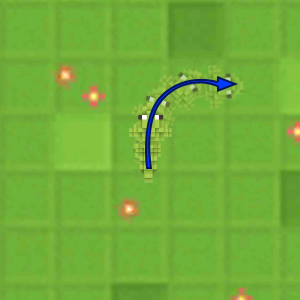
\includegraphics[width=0.3\textwidth]{SnakeDirection1}
	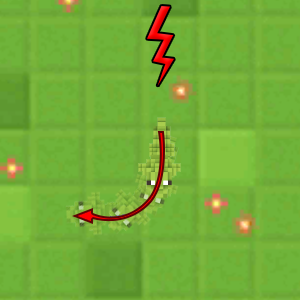
\includegraphics[width=0.3\textwidth]{SnakeDirection2}
	\caption{Links: Pfeiltaste nach rechts = nach rechts bewegen. Rechts: Pfeiltaste nach rechts = nach links bewegen\label{fig:controlIssue}}
\end{figure}
\section{Startpunktzahl}
\label{sec:startpointsDisk}
Am Anfang hatte jeder Spieler direkt 10 Punkte ohne einen Apfel gegessen zu haben, dies hätte eigentlich nicht der Fall sein sollen, hat aber weitere Beobachtungen eingebracht. Viele der Kinder scheinen nicht bemerkt zu haben, dass sie direkt mit 10 Punkten starten und gingen davon aus, dass sie schon etwas geschafft haben. Wenn die Kinder direkt am Anfang die Schlange sich selbst fressen ließen, fühlten siesich trotzdem ermutigt, da sie zumindest 10 Punkte erreicht hatten.
\section{Zusammenfassung und Ausblick}
\label{sec:ausblickDisk}
In diesem Kapitel soll die Arbeit nochmals zusammengefasst werden und die Erweiterungsmöglichkeiten des Spiels, sowie mögliche weitere Studien diskutiert werden.\\
\\
Insgesamt wurde die Zielsetzung dieser Arbeit, ein Mathelernspiel, zum erlernen der Addition, zu entwicklen, erfüllt. Das Spiel wurde in der Entwicklungsumgebung von Unity entwickelt, die als Einsteiger gut erlernbar ist. Damit konnte ich ein, durch den anschließenden Nutzertest bestätigtes, tolles Mathespiel entwickeln. Evaluiert wurde das Spiel über den Kids-GEQ Nutzertest. Dieser ermöglichte mir es einzelne Kategorien gezielt auszuwerten und auf die Forschungsfragen eine Antwort zu bekommen. Da das Spiel mit für das Tablet entwickelt wurde, konnte ich das Spiel leicht mit den fünf Kindern testen. Durch diese Arbeit konnte ich zeichen, dass die beide Versionen den Kindern gefallen, aber sie die Third-Person Version bevorzugen. Dies wurde zusätzlich, zu den vom Kids-GEQ gesammelten Daten, auch von den schriftlichen Fragen am Ende des Nutzertests bestätigt. Alle Nutzer haben bei der Frage, welches Spiel ihnen mehr Spaß gemacht hat die Third-Person Variante angegeben. Als schwieriger wurde von vier der fünf Kinder die TopDown Variante genannt. Diese Schwierigkeiten hatten vor allem Auswirkungen auf das Flow- und Challenge-Ergebnis, wie bereits in den Kapiteln \ref{sec:flowDisk} und \ref{sec:challengeDisk} beschrieben wurde.\\
Insgesamt können beide Forschungsfragen, aufgrund der geringen Stichprobenmenge, nicht eindeutig beantwortet werden. Allerdings kann anhand der Tendenzen gesagt werden, dass ein solches Lernspiel zur Unterstützung der Addition über Partnerzahlen den Kindern mit hoher Wahrscheinlichkeit Spaß bereitet. Außerdem konnte eine starke Tendenz zur Third-Person Variante erkannt werden. Ob diese nach Behebung einiger Schwierigkeiten der TopDown-Perspektive bestehen bleibt, ist durch zukünftige Tests zu ermitteln. Auch die generelle Wirksamkeit des Spiels ist durch weitere Nutzertests zu untersuchen.\\
\\
Das Spiel MathSnake lässt sich noch in vielen Bereichen verbessern. Eine Verbesserung im Design und den visuellen Effekten wäre, für die Third-Person Version den Kamerafehler am Ende einer Spielrunde zu entfernen. Es wäre hier interessant zu sehen ob das verzerrte Bild am Ende der Spielrunde negative Einflüsse auf das Spielgefühl bewirkt. Ein weiterer wichtiger Punkte ist, für die TopDown Version der Kontrast der Schlange. Dieser wurde mehrheitlich unter den Nutzern als verbesserungswürdig eingestuft. Da in dem verwendeten Asset-Pack mehrere Schlangendesigns enthalten sind, könnte der Spieler hier am Anfang des Spiels seine Schlange wählen. Dies könnte den Effekt haben, dass der Spieler sich auch gleichzeitig mehr mit seiner Spielfigur identifizieren kann und somit die wahrgenommene Autonomie, ein wichtiger Aspekt intrinischer Motivation\cite{Deci2000TheW}, addressiert werden könnte. Für einen vielleicht steigenden Immersions-Wert könnte zusätzlich sorgen, wenn die Grafik für den Boden überarbeitet werden, damit diese ebenso scharf dargestellt wird wie der Rest der Spielwelt.\\
\\
Auch für einen höheren Challenge-Wert kann das Spiel optimiert werden. So wäre es zum Beispiel möglich, das Spiel auch für höhere Klassenstufen interessanter zu gestalten. Der Anstieg der Schwierigkeitsstufe auf ein Level mit verfaulenden Äpfeln wurde für diesen Nutzertest so weit nach oben gesetzt, dass kein Spieler dieses Level erreichte. Das war für diese Altersgruppe aber auch nicht vorgesehen. In neueren Versionen kann also das Levelsystem angepasst werden, um auch zu diesem Level, nach einer angemessenen Spielzeit zu kommen. Auch mögliche Erweiterungen des Levelsystems wurden festgehalten. So ist es möglich weitere Level einzufügen in denen zum Beispiel 'Fake-Äpfel' auftauchen. Dies sind Äpfel, die dem Spieler effektiv nicht helfen die gesuchte Zahl zu bilden. Das heißt sie sollten von der Schlange nicht gegessen werden. Damit sind auch weitere Erweiterungen möglich, die die Schlange fressen kann. So ist es dann auch möglich ein Item einzuführen, welches diese 'Fake-Äpfel' identifizieren kann oder andere Eigenschaften mit sich bringt, wie Items die die Schlange verkürzen oder verlangsamen, aber auch Items mit denen der Spieler die zu suchende Zahl ändern kann als eine Art Joker.\\
\\
Es wäre auch interessant nicht nur die Addition zu untersuchen, sondern auch andere mathematische Operatoren. So könnte durch das einfache Hinzufügen von \qq{Operator-Äpfeln} die Komplexität und damit ebenfalls der Challenge-Faktor deutlich erhöht werden. Mit diesen speziellen Äpfeln wäre es außerdem möglich die Aufgabe an den Spieler zu varriieren. So kann er in einem Level ganz normal die Partnerzahlen suchen und in einem anderen sind die Zahlen der Gleichung vielleicht schon gegeben und er muss nur die richtigen Operatoren der Reihe nach einfügen. Im Gleichungsbereich könnte so etwas stehen wie $10 = 10   10   10$ und der Spieler bekommt Äpfel für die Multiplikation und Division.\\
\\
Auch für den Nutzertest sind Verbesserungen möglich. Indem eine größeren Stichprobenmenge verwendet wird, aber auch weitere Fragen können durch Nutzertests beantwortet werden. So zum Beispiel, ob Startpunkte, wie in Unterkapitel\ref{sec:startpointsDisk} beschrieben, den Wert der positiven Effekte steigert oder unerheblich für diesen ist. Außerdem wurde, wie in Unterkapitel \ref{sec:tensionDisk} beschrieben, ein Problem mit der Steuerung der TopDown Variante festgestellt. Hier ist über Nutzertests zu überprüfen, ob eine Änderung der Steuerung zur klassischen Snake Variante sinnvoll wäre. Im klassischen Snake steuert der Spieler die Schlange mit allen Richtungstasten und gibt jeweils an, in welche Richtung sich die Schlange bewegen soll. Dabei sind ausschließlich $90^\circ$ Drehungen möglich.

%TODO schönen Schluss schreiben wenn noch Zeit